\documentclass[a4paper,10pt]{article}

\usepackage[T1]{fontenc}
\usepackage[utf8]{inputenc}
\usepackage[brazil]{babel}
\usepackage[skins,breakable]{tcolorbox}

\usepackage{geometry}
\geometry{
    textwidth=190mm,
    textheight=267mm,
	inner=10mm,
	outer=10mm,
	top=10mm,
	bottom=20mm
}
\usepackage{fancyhdr}
\usepackage{graphicx}
\usepackage{fontawesome}
\usepackage{hyperref}
\hypersetup{
	colorlinks = true,
	urlcolor = cyan,
	linkcolor = black,
}

%%%%%%%%%%%%%%%%%% - Alterações de Uso - %%%%%%%%%%%%%%%%%%
\newcommand{\profissional}{Mateus Souza Oliveira}
\newcommand{\idade}{26}
\newcommand{\Endereco}{Rodovia Amaro Antônio Vieira, 2593 -- Itacorubi. Florianópolis, Santa Catarina, Brasil}
\newcommand{\telefone}{+55 (48) 9 9810-2694}
\newcommand{\email}{matews1943@gmail.com}
\newcommand{\data}{\today}
\newcommand{\sobre}{
    Pró-ativo, detalhista, determinado e sempre em busca de me aprimorar. Atualmente, estou trabalhando como desenvolvedor web. Tenho experiência com Python, Git, Docker, SQL, Linux, JavaScript, Testes, ferramentas de qualidade de código, Integração Contínua, PostgreSQL e GitHub, GitLab e Bitbucket. Sou fluente em inglês.\\

    Tenho interesse em trabalhar com Python e automatizações. Prefiro trabalhar com Linux.
}
%%%%%%%%%%%%%%% - Fim de Alterações de Uso - %%%%%%%%%%%%%%

\setlength{\fboxrule}{2pt}
\setlength{\fboxsep}{0pt}

\fancyhead{} % Cabeçalho: reset
\fancyfoot{} % Rodapé: reset
\fancyfoot[C]{Página \thepage \ de \pageref{ultimaPagina}} % Rodapé: centro
\fancyfoot[R]{Feito com \LaTeX} % Rodapé: direito
\fancyfoot[L]{Atualizado em \data} % Rodapé: esquerdo
\renewcommand{\headrulewidth}{0pt} % Espessura da linha de cabeçalho
\renewcommand{\footrulewidth}{0.4pt} % Espessura da linha de rodapé
\pagestyle{fancy} % Define o estilo da página

\newcommand{\criaSecao}[4][0]{
	\begin{tcolorbox}[
        blanker,
        breakable,
        title=\begin{minipage}{0.16\linewidth}\large{\textbf{#2}}\vspace{-#3\baselineskip}\end{minipage},
        coltitle=black,
        leftupper=0.21\linewidth,
    ]
        #4
		\ifnum0#1>0 { \hrule {\ } } \fi
    \end{tcolorbox}
}

\begin{document}

	\noindent
	\fbox{
	\hspace*{-3.35\fboxrule}
	\begin{minipage}{0.3\linewidth}
		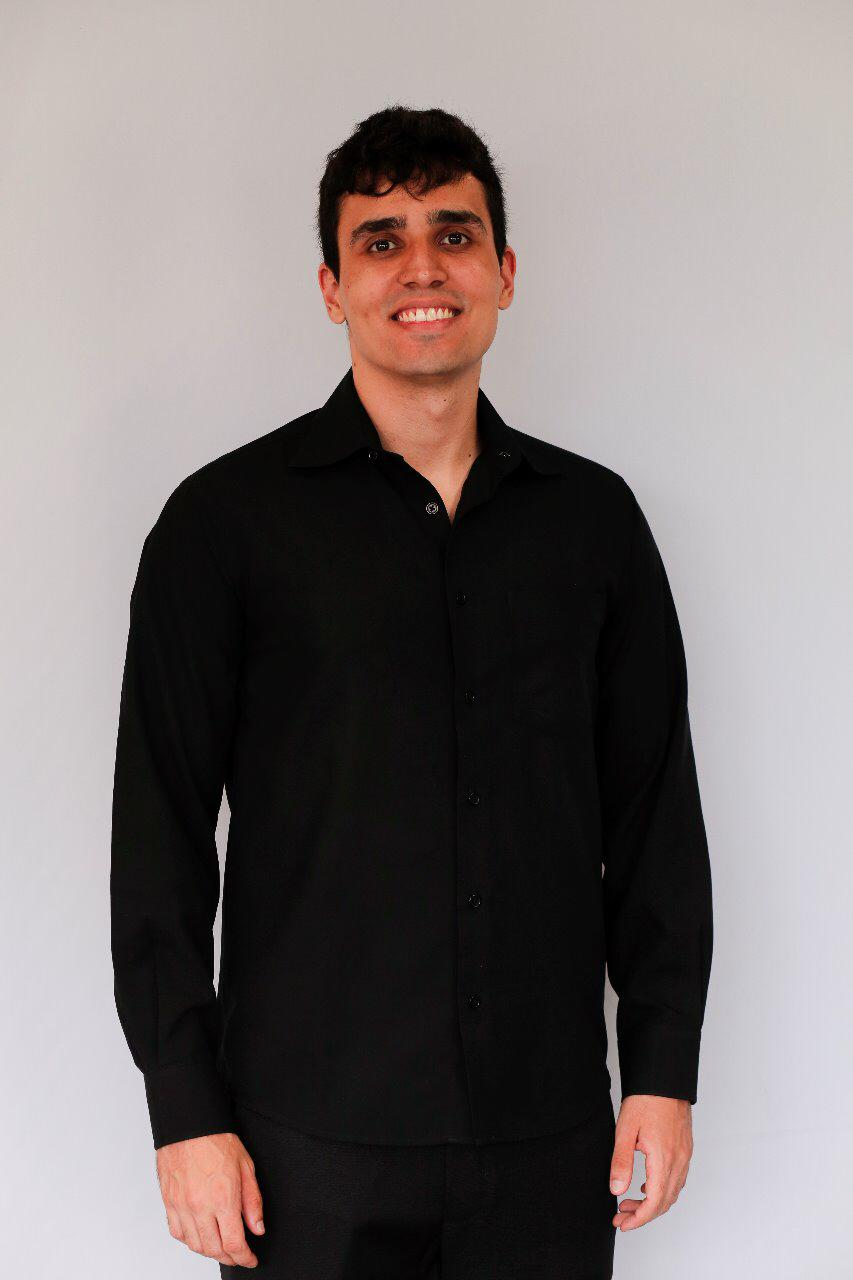
\includegraphics[width=\linewidth]{img/profile.jpeg}
	\end{minipage}
	\hspace*{-3.35\fboxrule}
	}
	\hfill
	\begin{minipage}{0.65\linewidth}
		\Huge{\bf \profissional, \idade}\\\vspace{-1.75\baselineskip}

		\noindent\rule{\textwidth}{1.5pt} {\ }\\\vspace{-1.8\baselineskip}

		\large{
		\faMapMarker \ \Endereco \\
		\begin{minipage}{0.5\linewidth}
			\faWhatsapp \ \telefone
		\end{minipage}
		\begin{minipage}{0.5\linewidth}
			\faEnvelope \ \email
		\end{minipage}
		\begin{minipage}{0.5\linewidth}
			\faLinkedinSquare \ \href{https://www.linkedin.com/in/mateusoliveira43/}{\texttt{/mateusoliveira43}}
		\end{minipage}
		\begin{minipage}{0.5\linewidth}
			\faGithub \ \href{https://github.com/mateusoliveira43}{\texttt{/mateusoliveira43}}
		\end{minipage}
		\faLink \ \href{https://mateusoliveira43.github.io/}{\texttt{mateusoliveira43.github.io}}\\
		\vfill
		\textbf{Sobre}:\sobre
		}
	\end{minipage}
	\vspace{\baselineskip}

%%%%%%%%%%%%%%%%%%%%% - Corpo do CV - %%%%%%%%%%%%%%%%%%%%%
    \criaSecao[1]{Educação}{2}{
		\textit{Matemática - Bacharelado}, Universidade Federal de Santa Catarina (UFSC), Florianópolis, Santa Catarina \hfill 2014 - 2020 \\
    }

    \criaSecao[1]{Experiência}{2}{
        \textit{Desenvolvedor de Software Júnior}, Fundação CERTI, Florianópolis, Santa Catarina \hfill Outubro 2020 - atualmente \\
        Maio 2022 - Atualmente\\
        \textbf{Atividades}: Manutenção de Framework Python, de empresa Alemã, para testes em dispositivo real e simulado e escrita de novos testes. Estrutura do cliente sendo o GitLab.\\

        Atuei na criação da estrutura de integração contínua do projeto, implementação de suas métricas de qualidade, conteinerização com Docker e implementação da estrutura de colocar a documentação do projeto no ar.\\

        Março 2022 -  Abril 2022\\
        \textbf{Atividades}: Atualização do site interno da Fundação CERTI para trocar o uso de PHP e Vue.js para Node.js e React (e TypeScript).\\

        Atuei na criação da nova estrutura do backend do site, de sua estrutura de integração contínua, implementação de suas métricas de qualidade, conteinerização com Docker.\\

        Outubro 2020 - Fevereiro 2022\\
        \textbf{Atividades}: Projeto WEB e aplicativo desktop (além da tradução do código de cálculos em Visual Basic para Python), de empresa nacional, envolvendo Python (PyPy, FastAPI, SQLAlchemy, Numpy, Pandas) no Backend, JavaScript (TypeScript, Node.js, React) no Frontend, PostgreSQL no banco de dados. Todo o código tendo integração contínua através do Jenkins, métricas de qualidade com testes, linter e SonarQube e conteinerizado com Docker.\\

        Atuei na criação da estrutura do frontend do site, definição da estrutura do banco de dados (junto com o cliente e time de engenharia mecânica/petróleo), revisões e implementações (tanto no backend quanto no frontend) e automatizações. Além disso, fui uma das lideranças do time (que contava com equipes de desenvolvimento, QA, UX e engenharia mecânica/petróleo). Planejamento e trabalho seguindo alguns princípios de metodologia ágeis.\\

        Agosto 2021 - Janeiro 2022\\
        \textbf{Atividades}: Projeto legado embarcado Linux com interface WEB (IHM), de empresa Alemã, envolvendo C++ no dispositivo, JavaScript (Meteor) no Backend e Frontend, SQLite no banco de dados. Código tendo integração contínua através do GitLab, métricas de qualidade com testes, linter e conteinerizado com Docker.\\

        Atuei implementando melhorias na integração contínua dos repositórios e melhorias e automatizações com Python. Planejamento e trabalho em inglês.\\

        \textit{Bolsista de Iniciação Científica}, Universidade Federal de Santa Catarina (UFSC), Florianópolis, Santa Catarina \hfill Agosto 2019 - Fevereiro 2020 \\
		\textbf{Atividades}: Pesquisa voltada a computação gráfica.\\

		\textit{Bolsista do Laboratório de Estudos de Matemática e Tecnologias}, Universidade Federal de Santa Catarina (UFSC), Florianópolis, Santa Catarina \hfill Março 2019 - Julho 2019 \\
		\textbf{Atividades}: Aplicação, desenvolvimento e atualização de arquivos do projeto.\\

		\textit{Bolsista da Revista da Olimpíada Regional de Matemática de Santa Catarina}, Universidade Federal de Santa Catarina (UFSC), Florianópolis, Santa Catarina \hfill Março 2016 - Março 2017 \\
		\textbf{Atividades}: Aplicação e desenvolvimento de arquivos de treinamento; correção e desenvolvimento de arquivos de prova; atualização do arquivo mestre da revista.\\

		\textit{Bolsista do Programa de Educação Tutorial de Matemática}, Universidade Federal de Santa Catarina (UFSC), Florianópolis, Santa Catarina \hfill Março 2015 - Fevereiro 2016 \\
		\textbf{Atividades}: Aplicação e desenvolvimento de arquivos de treinamento; lecionamento em cursinho pré-vestibular; lecionamento e elaboração de minicursos de \LaTeX\ e Matlab. \\
    }

    \criaSecao[1]{Linguagens de programação e ferramentas}{4}{
        \large{\bf
			\begin{minipage}{0.65\linewidth}
				Python (FastAPI, pytest, unittest, argparse)\\
				JavaScript (TypeScript, Node.js, React, Jest)\\
				Docker (Docker Compose)\\
				Linux\\
				GitHub\\
				Bitbucket\\
				PostgreSQL\\
			\end{minipage}
			\begin{minipage}{0.35\linewidth}
				Git\\
				SQL\\
				HTML\\
				CSS (Bootstrap)\\
				GitLab\\
				Jenkins\\
				\vspace{\baselineskip}
			\end{minipage}
		}
    }

	\criaSecao{Idiomas}{2}{
	    \large{
			\begin{minipage}{0.5\linewidth}
				\textbf{Português}: nativo \\
				\textbf{Inglês}: fluente \\
				\textbf{Francês}: básico \\
			\end{minipage}
			\begin{minipage}{0.5\linewidth}
				\textbf{Espanhol}: básico \\
				\textbf{Alemão}: básico \\
				\vspace{\baselineskip}
			\end{minipage}
		}
	}
%%%%%%%%%%%%%%%%%% - Fim do Corpo do CV - %%%%%%%%%%%%%%%%%
    \label{ultimaPagina}
\end{document}
